\label{chapter:metodo}
\section{Visão geral do método proposto}
   
O sistema computacional proposto será estruturado em forma de boia aquática, que será composta com microcontroladores, sensores para análise da água e para a captura ótica, visando adquirir imagens subaquáticas em tempo real. O sistema proposto contará com um módulo de classificação em uma central conectada, onde os dados serão processados e exibidos para o usuário final. 

A interação com a Boia (ainda me desenvolvimento), será através de uma conexão sem fio, como pode ser visto na \autoref{fig:bigpic}, visando mais praticidade para o usuário final, assim como facilidade de transporte da Boia, uma vez que a Boia pode ser energizada utilizando um painel solar.

 
   
%O sistema terá um sensor de captura ótica, que ficará submersos em água, acoplados à uma boia, que terá um conexão sem fio com um celular ou computador.

\begin{figure}[ht]
	\centering
    \caption{\label{fig:bigpic}Visão Geral}
	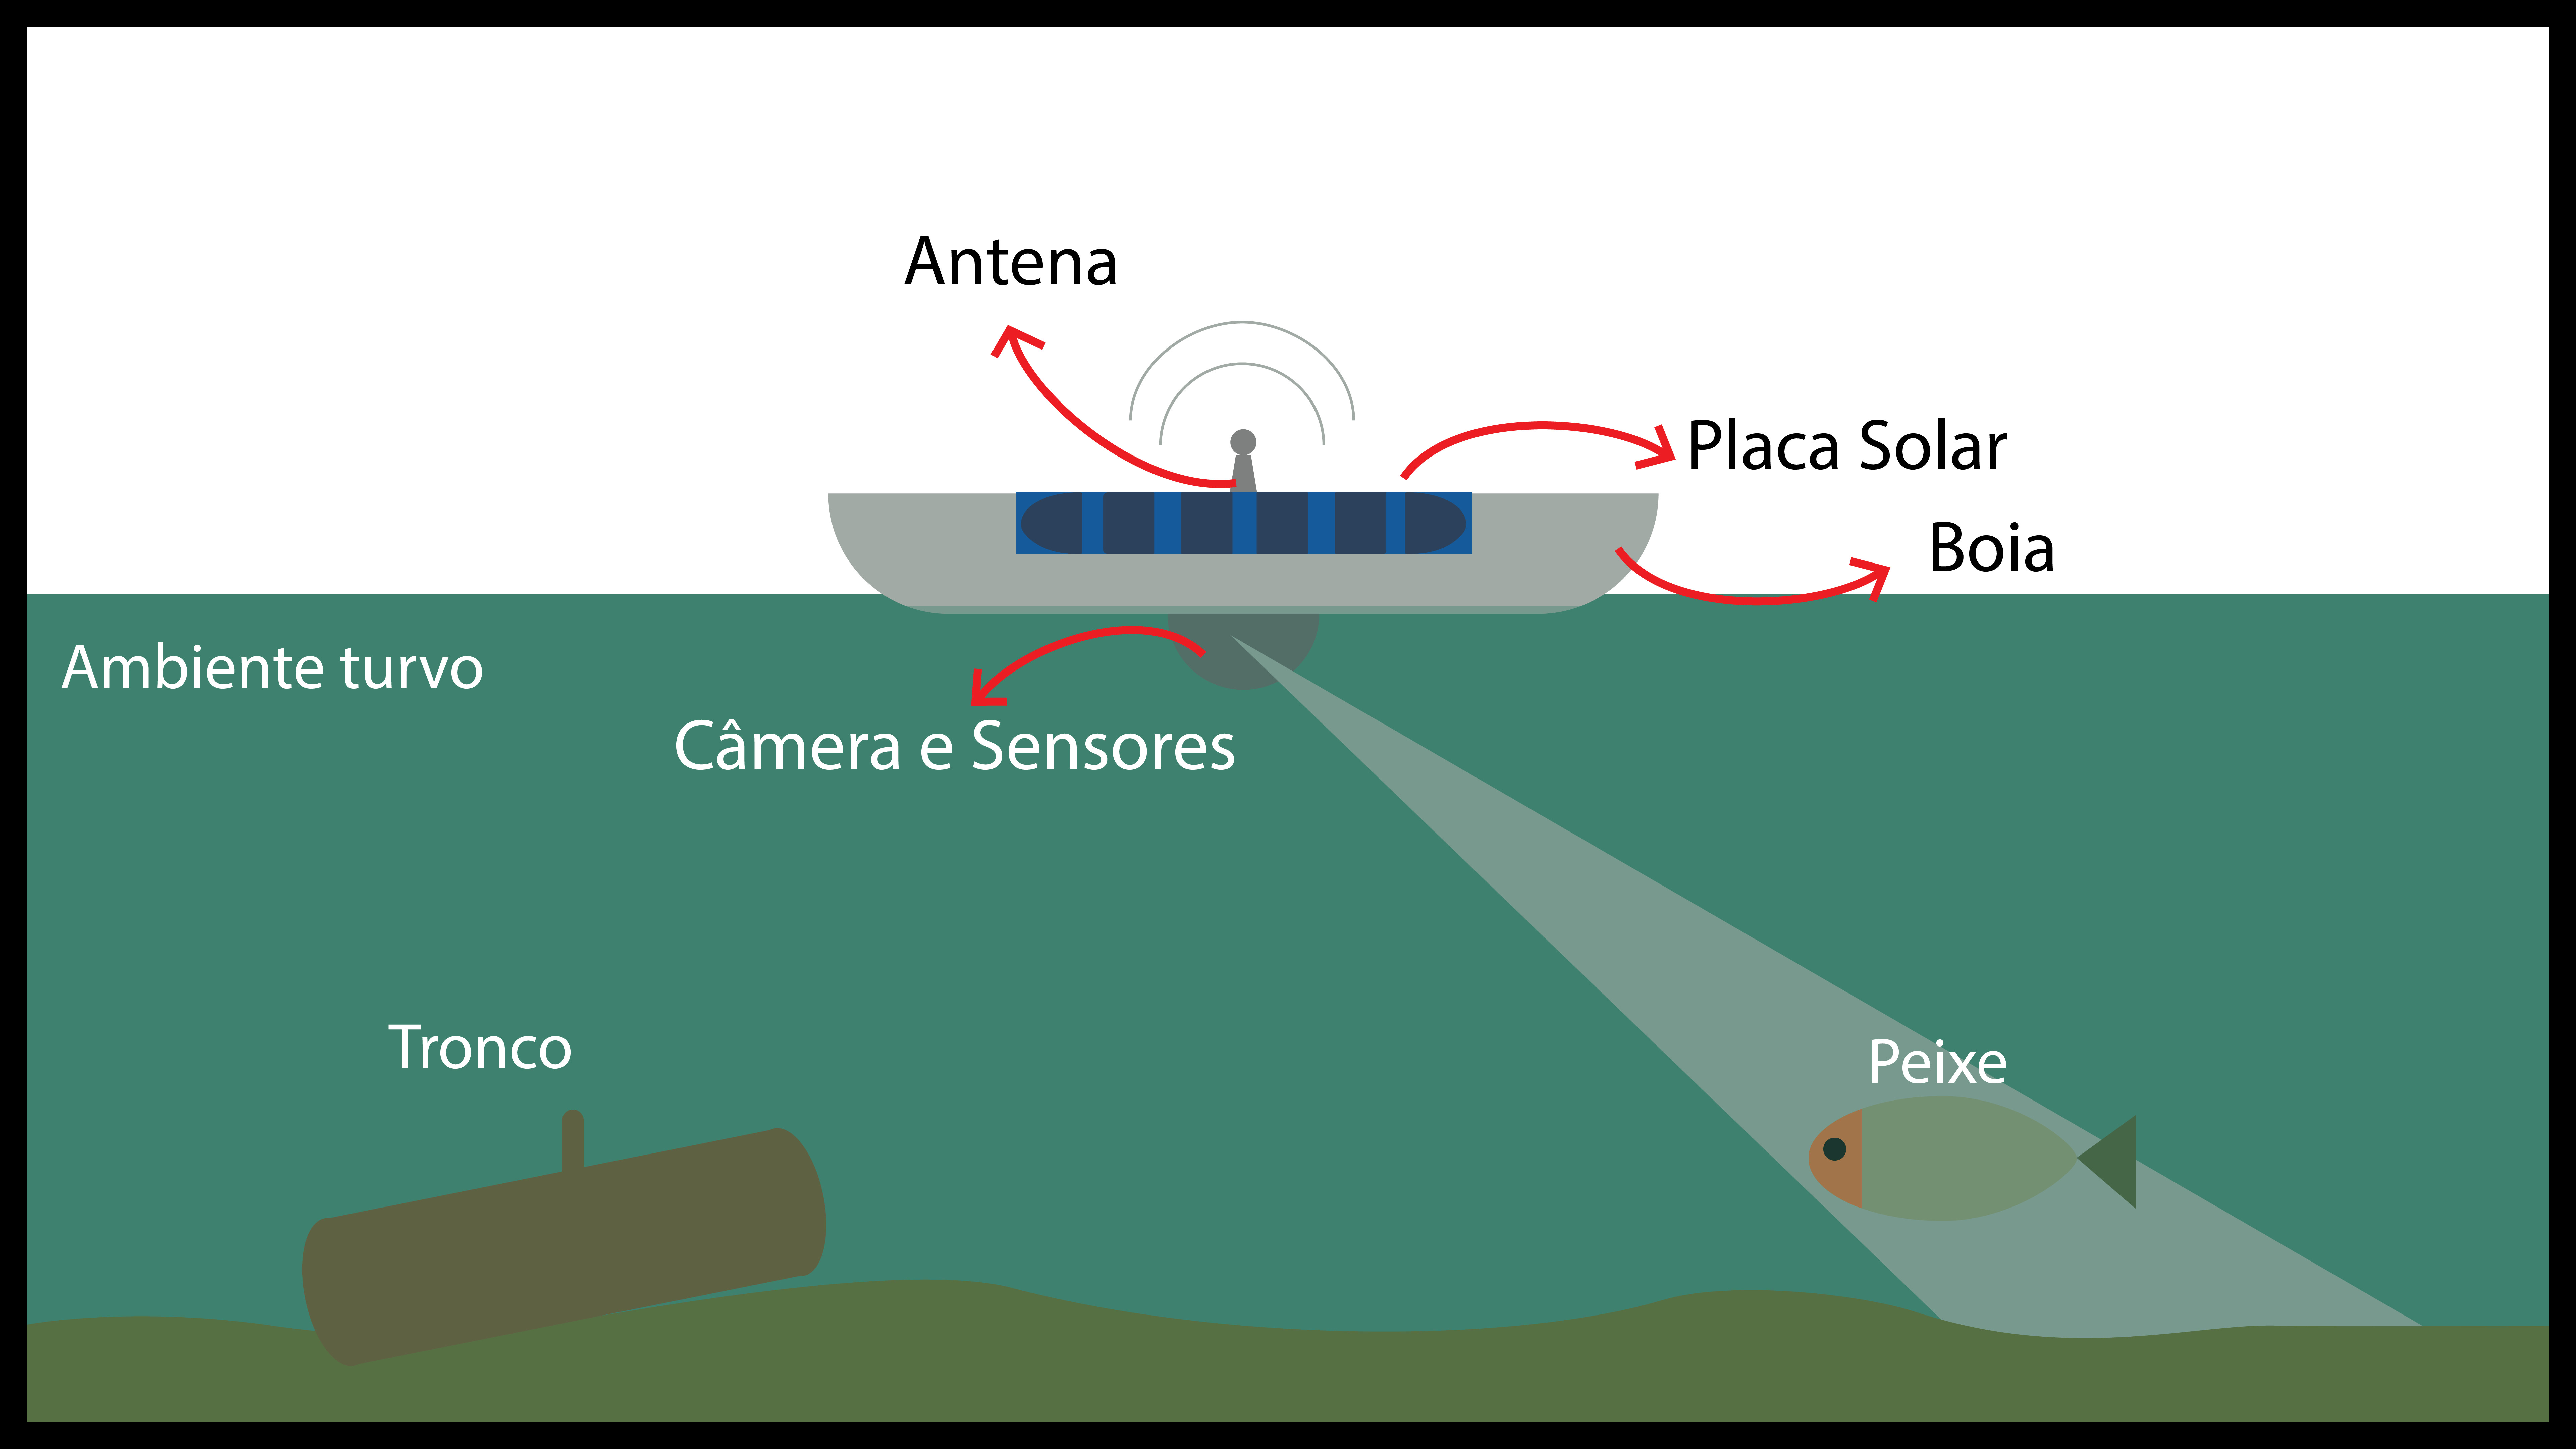
\includegraphics[width = \textwidth]{resources/bugpicturefloater}
    \legend{Fonte Própria}
\end{figure}

Na \autoref{fig:bigpic}, podemos ver como será o funcionamento do sistema computacional proposto em uma situação hipotética, e na \autoref{fig:storyb}, podemos ver como será feita a interação da Boia com a Central, mostrando suas etapas e telas. 

\section{Sistema computacional de suporte a coleta de imagens em ambientes fluviais: Kraken}
%\todo{o que será a boia;
%que sensores irá utilizar;
%como será a conexão com a centra;
%como será a centra;
%falar sobre a possibilidade de adição de sensores;}


A Boia proposta contará com microcontroladores que serão responsáveis por gerenciar os sistemas integrados à mesma, como motores e/ou estabilizadores e sensores para detecção de objetos e captura de imagens dentro do ambiente fluvial com alta turbidez, identificando objetos, classificando-os e especulando seu tamanho. A Boia servirá para facilitar muitas atividades, por exemplo, a prática de mergulho em áreas de risco, onde a visibilidade é quase nula.

A utilização de uma plataforma de sistema integrada (\textit{Single Board Computer}) com uso de microprocessador, contendo várias entradas (digitais e analógicas), irá garantir o suporte para novas extensões como um oxímetro, que irá medir o nível de oxigênio na água. O uso do microprocessador será o meio para interligar a maioria dos sensores e fará a conexão com a central, garantindo que os dados sejam tratados e enviados ao usuário final.


\begin{figure}[ht]
	\centering
    \caption{\label{fig:storyb}\textit{Storyboard}}
	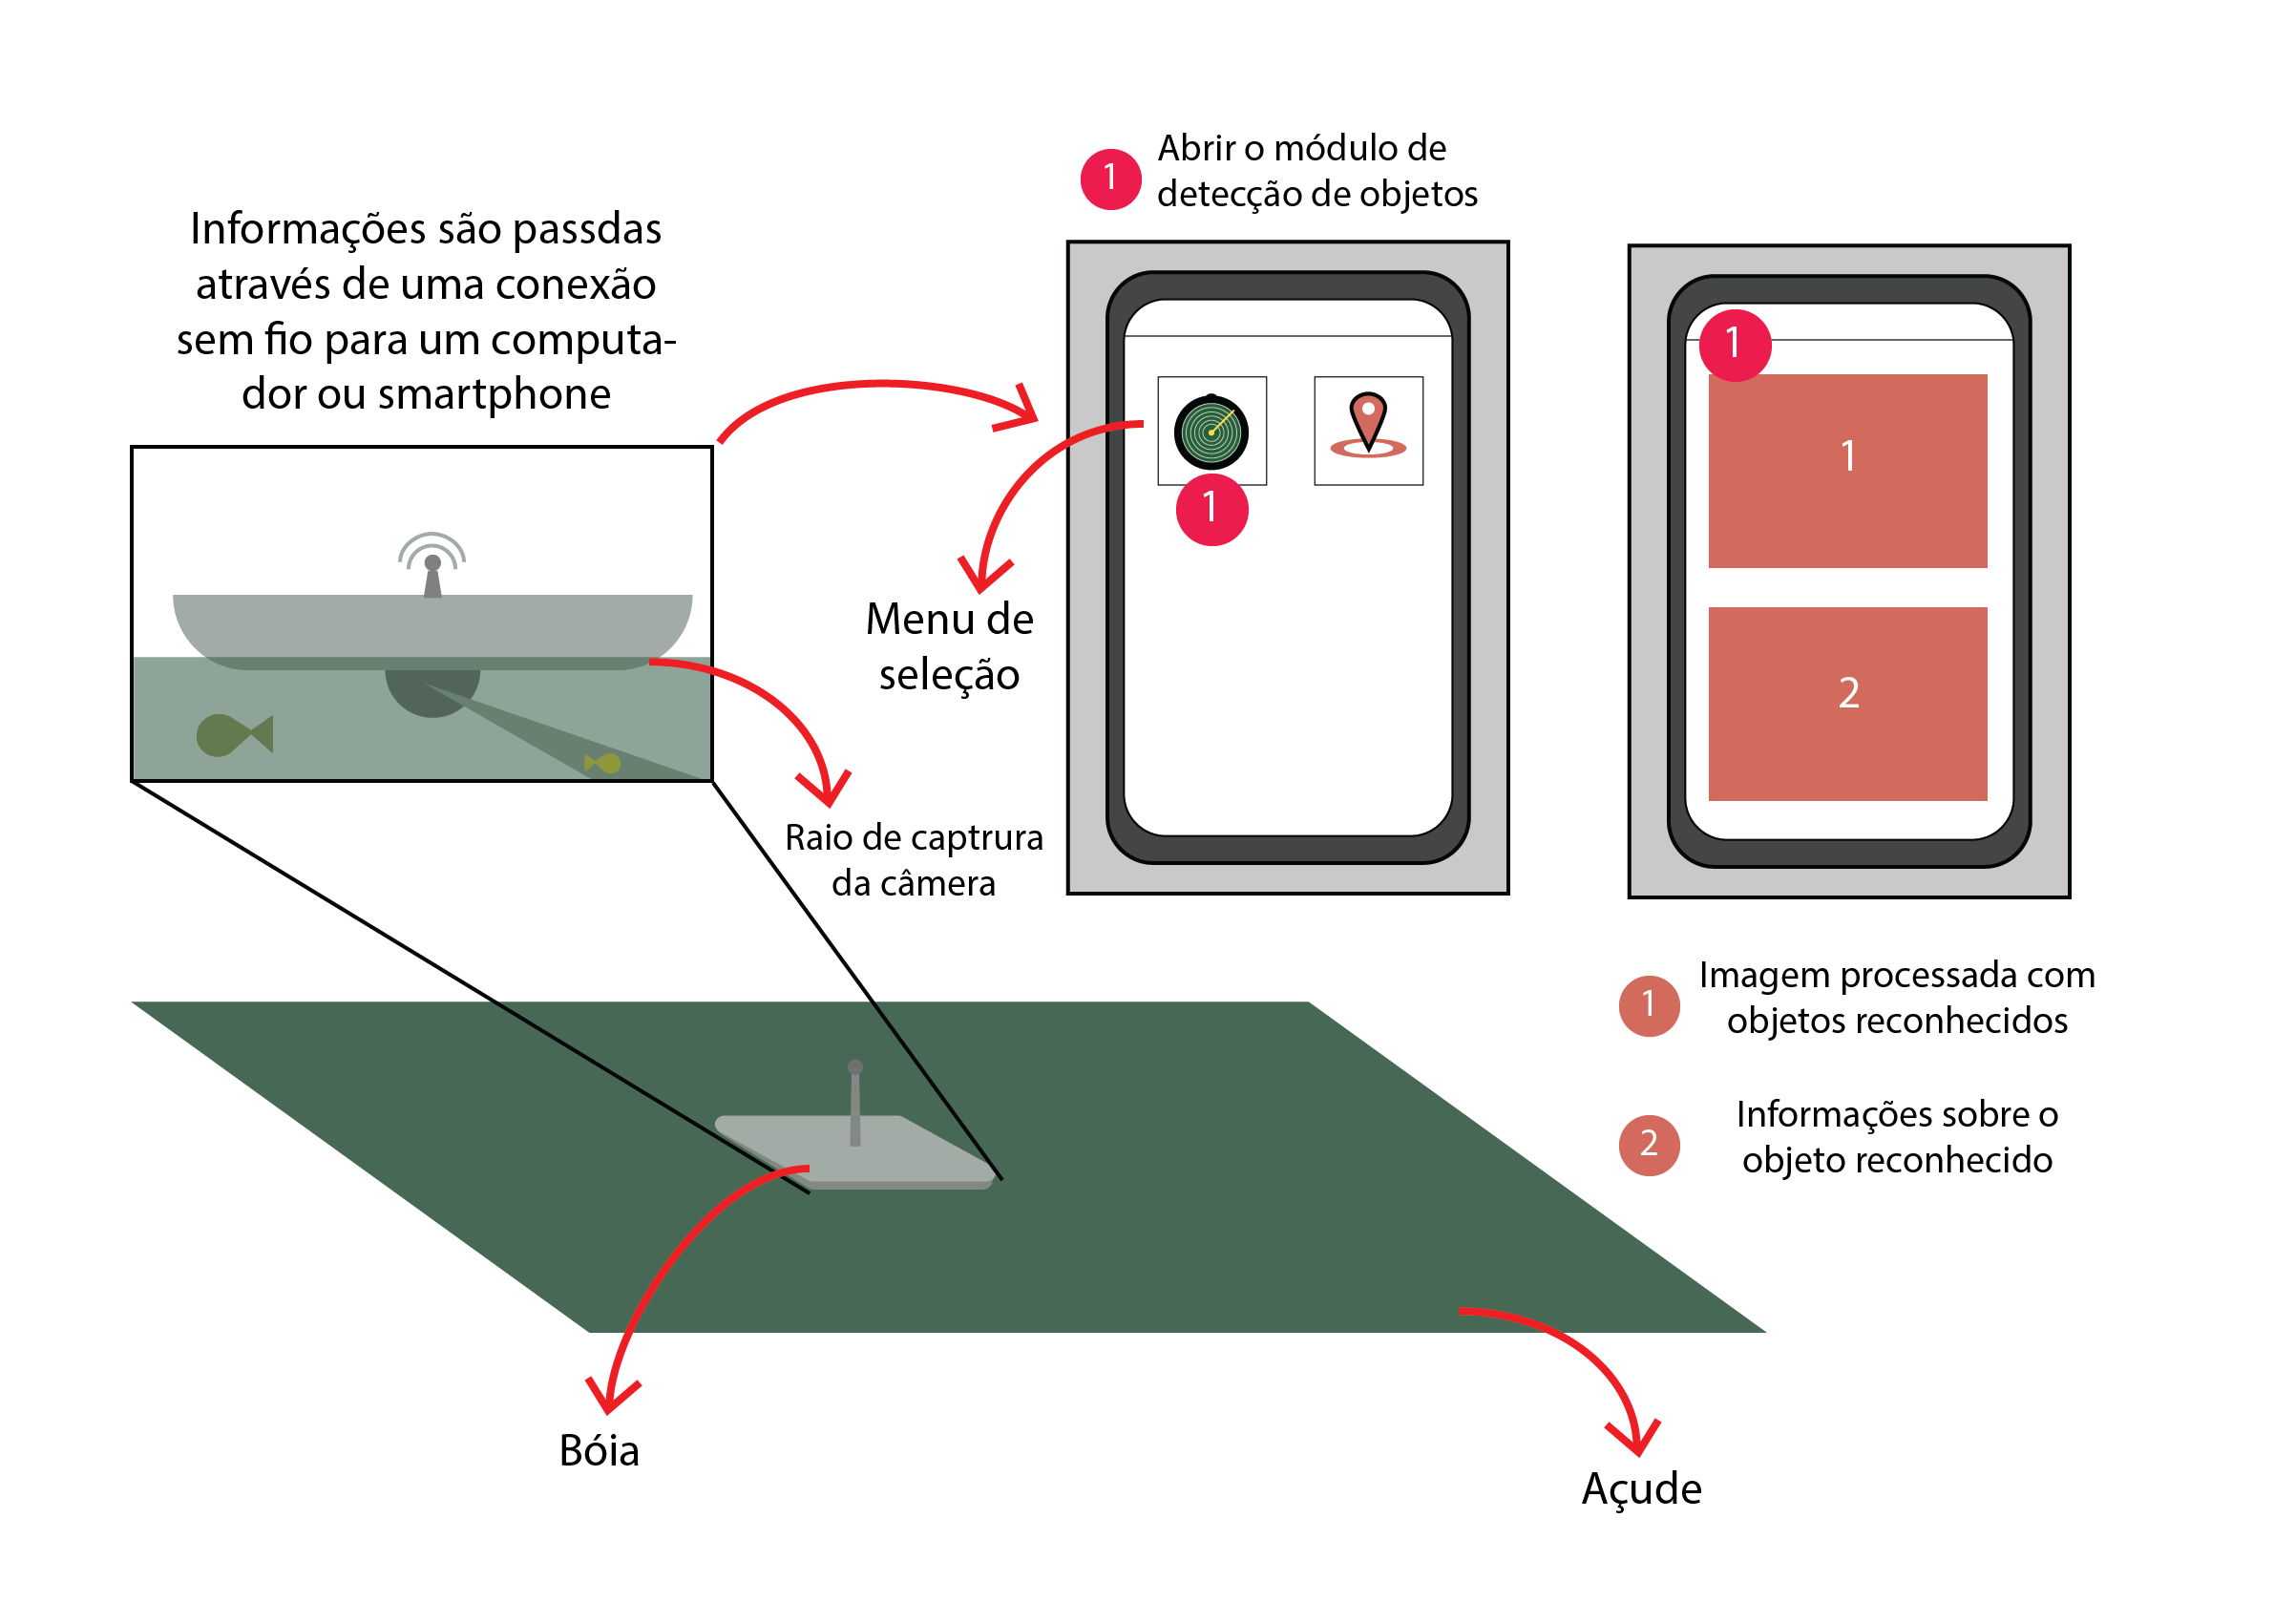
\includegraphics[width = 1 \textwidth]{resources/storyboard.png}
    \legend{Fonte Própria}
\end{figure}

A \autoref{fig:storyb} ilustra como serão as etapas de interação da Boia com a Central, que contará com um aplicativo de auxílio, onde serão exibidos os resultados para o usuário, tais como os dados coletados pela boia, garantindo uma entrega rápida de informação. 

Os dados classificados terão seus tamanhos especulados, e as imagens serão tratadas usando filtros com a biblioteca \textit{OpenCV}\cite{opencv}. A imagem será pré-processada antes de ser enviada ao classificador, isso irá garantir que a imagem esteja em perfeitas condições de classificação.


Além do aplicativo de auxilio, o sistema conta com um modulo de classificação de imagens que pode ser \textit{modelado} de acordo com a necessidade do ambiente, em especifico neste trabalho iremos adotar o \textit{framework Tensorflow}. 



\begin{figure}[ht]
	\caption{\label{fig:fluxcentral}  Fluxo de funcionamento do sistema proposto.}
	 \begin{center}
		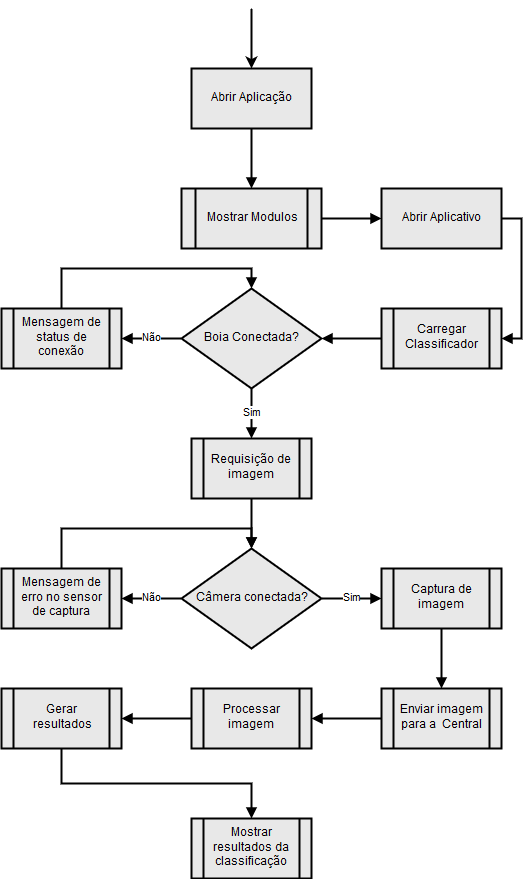
\includegraphics[width = 0.61\textwidth]			{resources/Fluxo-central}
    \end{center}
    \legend{Fonte Própria}
\end{figure}

Como demonstra a \autoref{fig:fluxcentral} o fluxo do sistema com a inicialização da aplicação, onde os módulos serão exibidos, dando opção para usuário abrir a aplicação para classificar e gerar o relatório da imagem. Em seguida a verificação se a Boia está conectada a Central e caso não esteja uma mensagem é retornada informando para o usuário que a conexão falhou, caso contrário, uma requisição de imagem é solicitada à Boia, onde mais uma vez será verificada a conexão com o sensor óptico, enviando mensagem de falha caso esteja desconectado. Uma vez que o a imagem é enviada para a Central, o módulo de classificação irá pré-processar a imagem caso seja necessário, e quando a imagem estiver adequada será processada e um relatório será gerado e exibido para o usuário.

O diagrama de sequência representeado pela \autoref{fig:seqkraken} mostra a sequência de interações do sistema, tais como: a interação do usuário com a Central; e da Central com a Boia. As condições caso haja falha nas conexões com os sensores e como proceder caso essas falhas sejam encontradas.

\begin{figure}[ht]
	\caption{\label{fig:seqkraken}  Diagrama de sequencia do sistema proposto.}
	 \begin{center}
		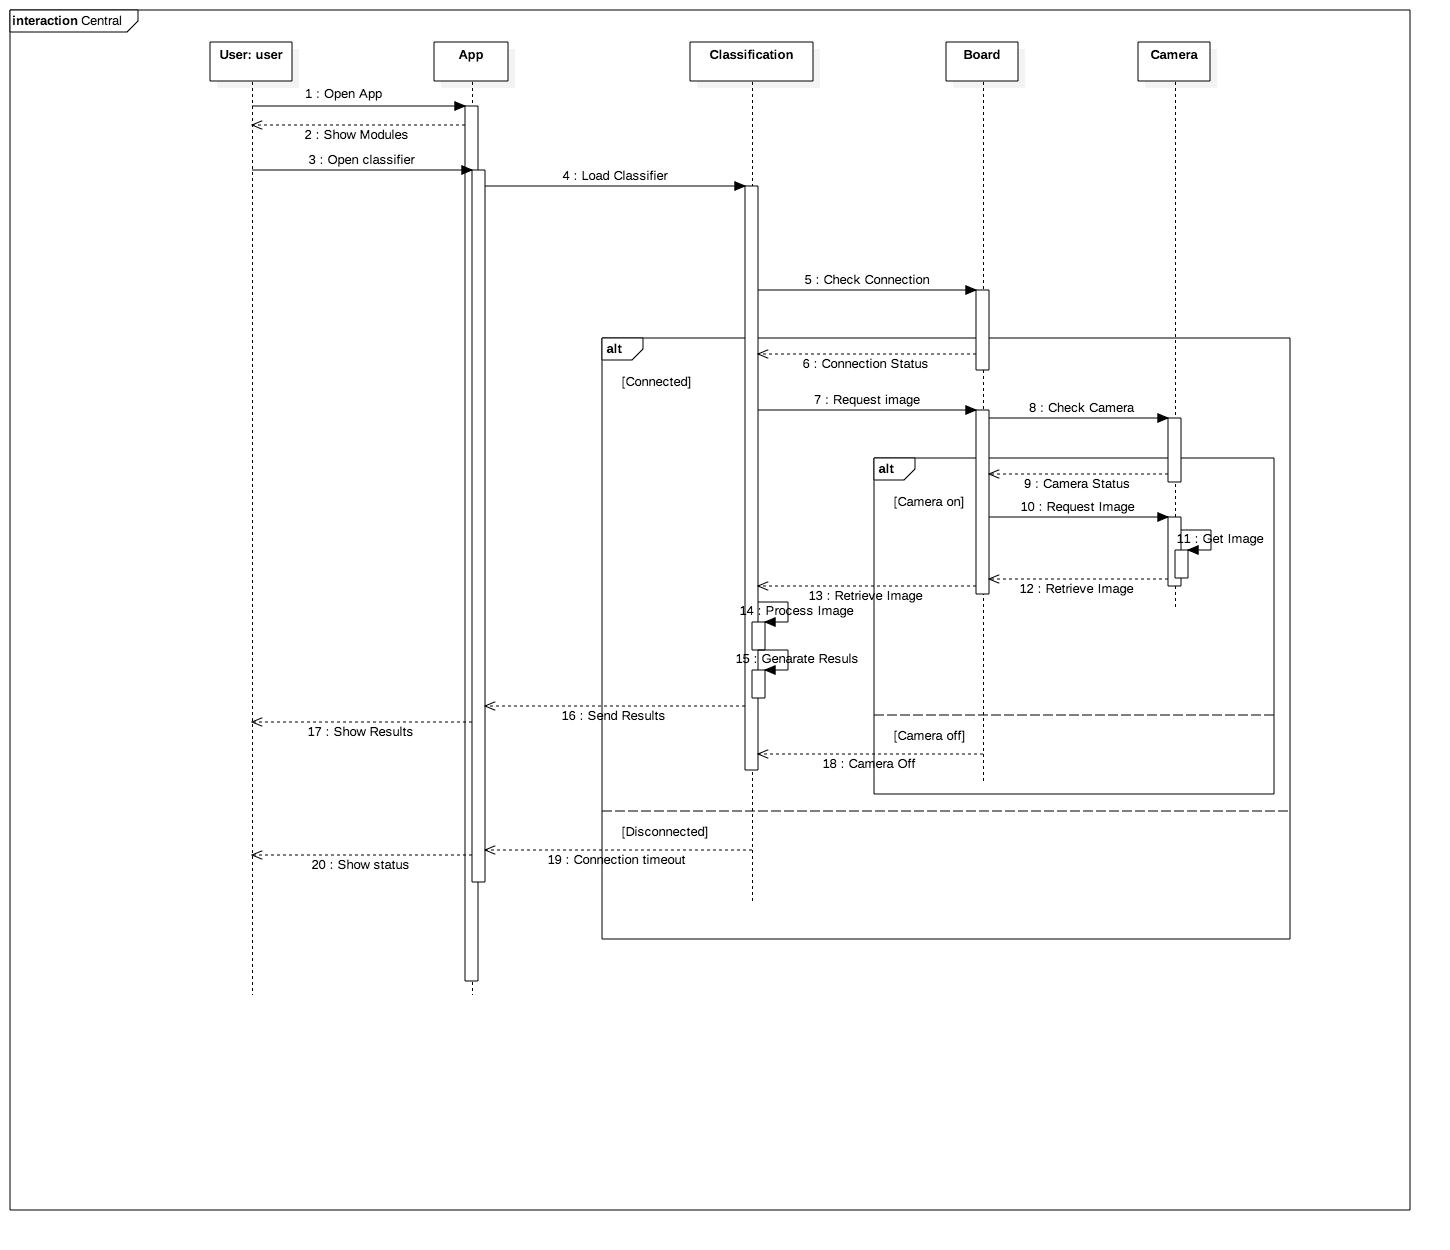
\includegraphics[width = 1\textwidth]			{resources/sequencekraken}
    \end{center}
    \legend{Fonte Própria}
\end{figure}

Detalhando o diagrama \autoref{fig:seqkraken}:
\begin{itemize}
    \item Usuário: o usuário receberá os \textit{feedbacks} através do aplicativo;
    \item Aplicativo: o aplicativo será responsável de entregar as mensagens para o usuário, e manusear a Central (conexão e sensores);
    \item Módulo de Classificação: Consiste em um módulo localizado na aplicação que será responsável por analisar, processar e classificar a imagem;
    \item Boia (Board / Câmera): A Boia que estará conectada à aplicação, onde estarão contidos os sensores e será responsável por adquirir imagens e as enviá-las. 
\end{itemize}


\section{Análise dos dados na central de processamento}

Como ilustra a \autoref{fig:fluxoprocesso}, após a coleta das imagens captados pelos sensores de captura (como câmeras) as imagens serão enviadas através de uma rede \textit{Wireless} para a Central, onde serão processados pelo módulo de Classificação que utilizará \textit{OpenCV} \cite{opencv} para os filtros de pré-processamento, afim de melhorar a qualidade da imagem coletada. A classificação é então executada nas imagens já processadas, usando o \textit{Tensorflow} que foi previamente modelado utilizando \textit{Inception}, para retreinar as últimas camadas da sua rede neural. 
% 
Após o processamento da imagem, será gerado um relatório sobre os dados processados dessa imagem e o resultado da classificação, exibindo um infográfico mostrando os resultados.

\begin{figure}[htbp]
	\centering
    \caption{\label{fig:fluxoprocesso}Fluxo de Processos do Sistema Computacional Proposto}
	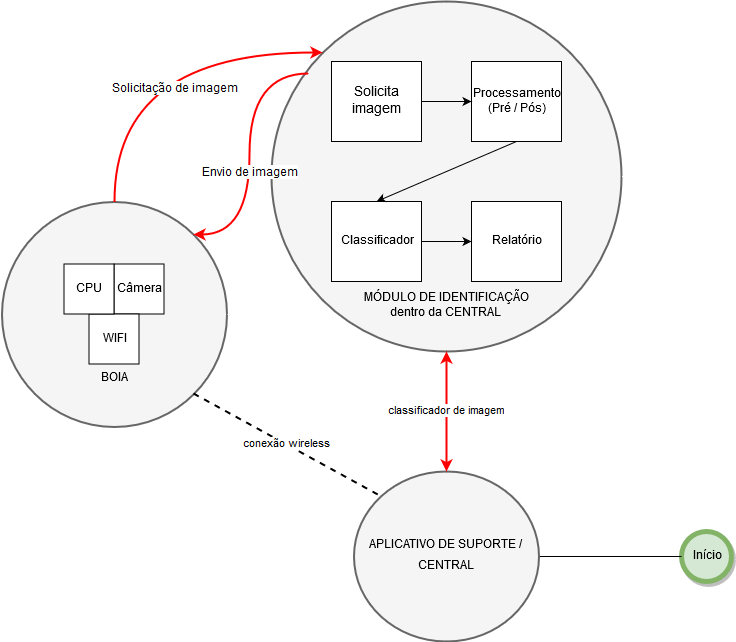
\includegraphics[width = 0.6\textwidth]{resources/fluxo-de-processo.png}
    \legend{Fonte Própria}
\end{figure}

\subsection{Pré processamento}
A etapa de pré-processamento consiste em verificar a qualidade da imagem para decidir se ela, vai passar por certas etapas de processamento para melhorias na imagem, caso a imagem esteja apta a classificação a mesma será enviada  deve ou não ser enviada para o módulo de pré-processamento. Dada a situação onde o ambiente observado não tem suas águas turvas o envio para o módulo de classificação


\begin{figure}[ht]
	\centering
    \caption{\label{fig:bigpic}Fluxo de Pré-processamento}
	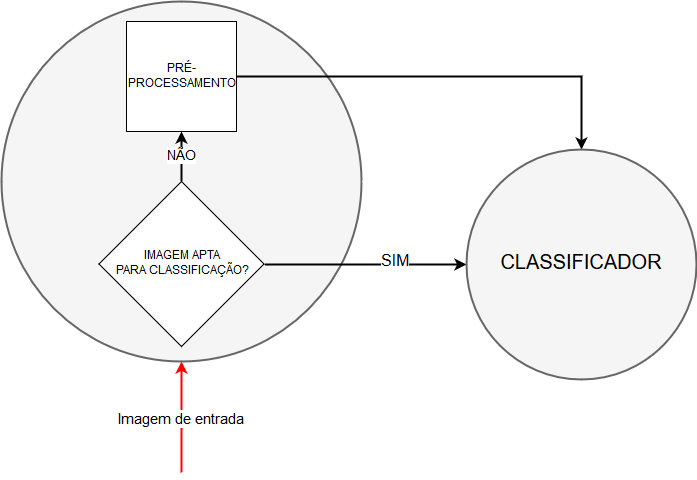
\includegraphics[width = 0.7\textwidth]{resources/fluxoprocessamento.png}
    \legend{Fonte Própria}
\end{figure}

\subsubsection{Filtro Homomórfico}
De acordo com \citeonline{bazeille2006}, o filtro homomórfico pode ser utilizado para corrigir os problemas de iluminação não uniforme e melhorar o contraste da imagem, aprimorando a nitidez da imagem ao mesmo tempo. Um exemplo do resultado da utilização pode ser visto na \autoref{fig:homomo}.

\begin{figure}[ht]
	\centering
    \caption{\label{fig:homomo}Resultado da utilização do filtro homomórfico no método do trabalho de \citeonline{bazeille2006}}
	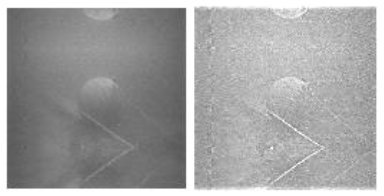
\includegraphics[width = 0.4\textwidth]{resources/homomo1.png}
    \legend{Adaptada de \citeonline{bazeille2006}}
\end{figure}
% \newpage


\subsubsection{Filtro Anisotrópico}
Segundo \citeonline{bazeille2006}, o filtro anisotrópico permite simplificar os atributos da imagem afim de aprimorar a segmentação da mesma, suavizando a imagem em uma área homogênea, preservando as arestas e as melhorando. Esse filtro é utilizado para remover alguns ruídos nas arestas causados pelo filtro homomórfico. Um exemplo da utilização do filtro pode ser visto na \autoref{fig:anisotop}. 

\begin{figure}[ht]
	\centering
    \caption{\label{fig:anisotop}Resultado da utilização do filtro anisotrópico método do trabalho de \citeonline{bazeille2006}}
	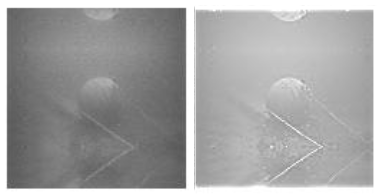
\includegraphics[width = 0.4\textwidth]{resources/anisitrop.png}
    \legend{Adaptada de \citeonline{bazeille2006}}
\end{figure}


%\section{Análise dos sensores}

 %Dada determinada situação onde a água não está com turbidez a utilização de um sensor pode detectar o ambiente e evitar que a central não necessite utilizar os filtros de pré-processamento nas imagens capturadas, melhorando o tempo de classificação.

%Com a possibilidade da adição de extensões à Boia, como sensores de medição de oxigenação da água, a necessidade de analise desses é algo pertinente para o desempenho da boia.



\section{Construção da Boia}

A estrutura da Boia, que é ilustrada na \autoref{fig:blueprint}, que visa baixo custo, utilizará materiais que podem ser encontrados com facilidade, como canos de PVC para a sustentação dos sensores e placas, tendo grande potencial para extensões ou modificações como alterar a estrutura para adicionar outro tipos de motores.

\begin{figure}[htbp]
	\centering
      \caption{\label{fig:blueprint} Descrição da construção da Boia.}
	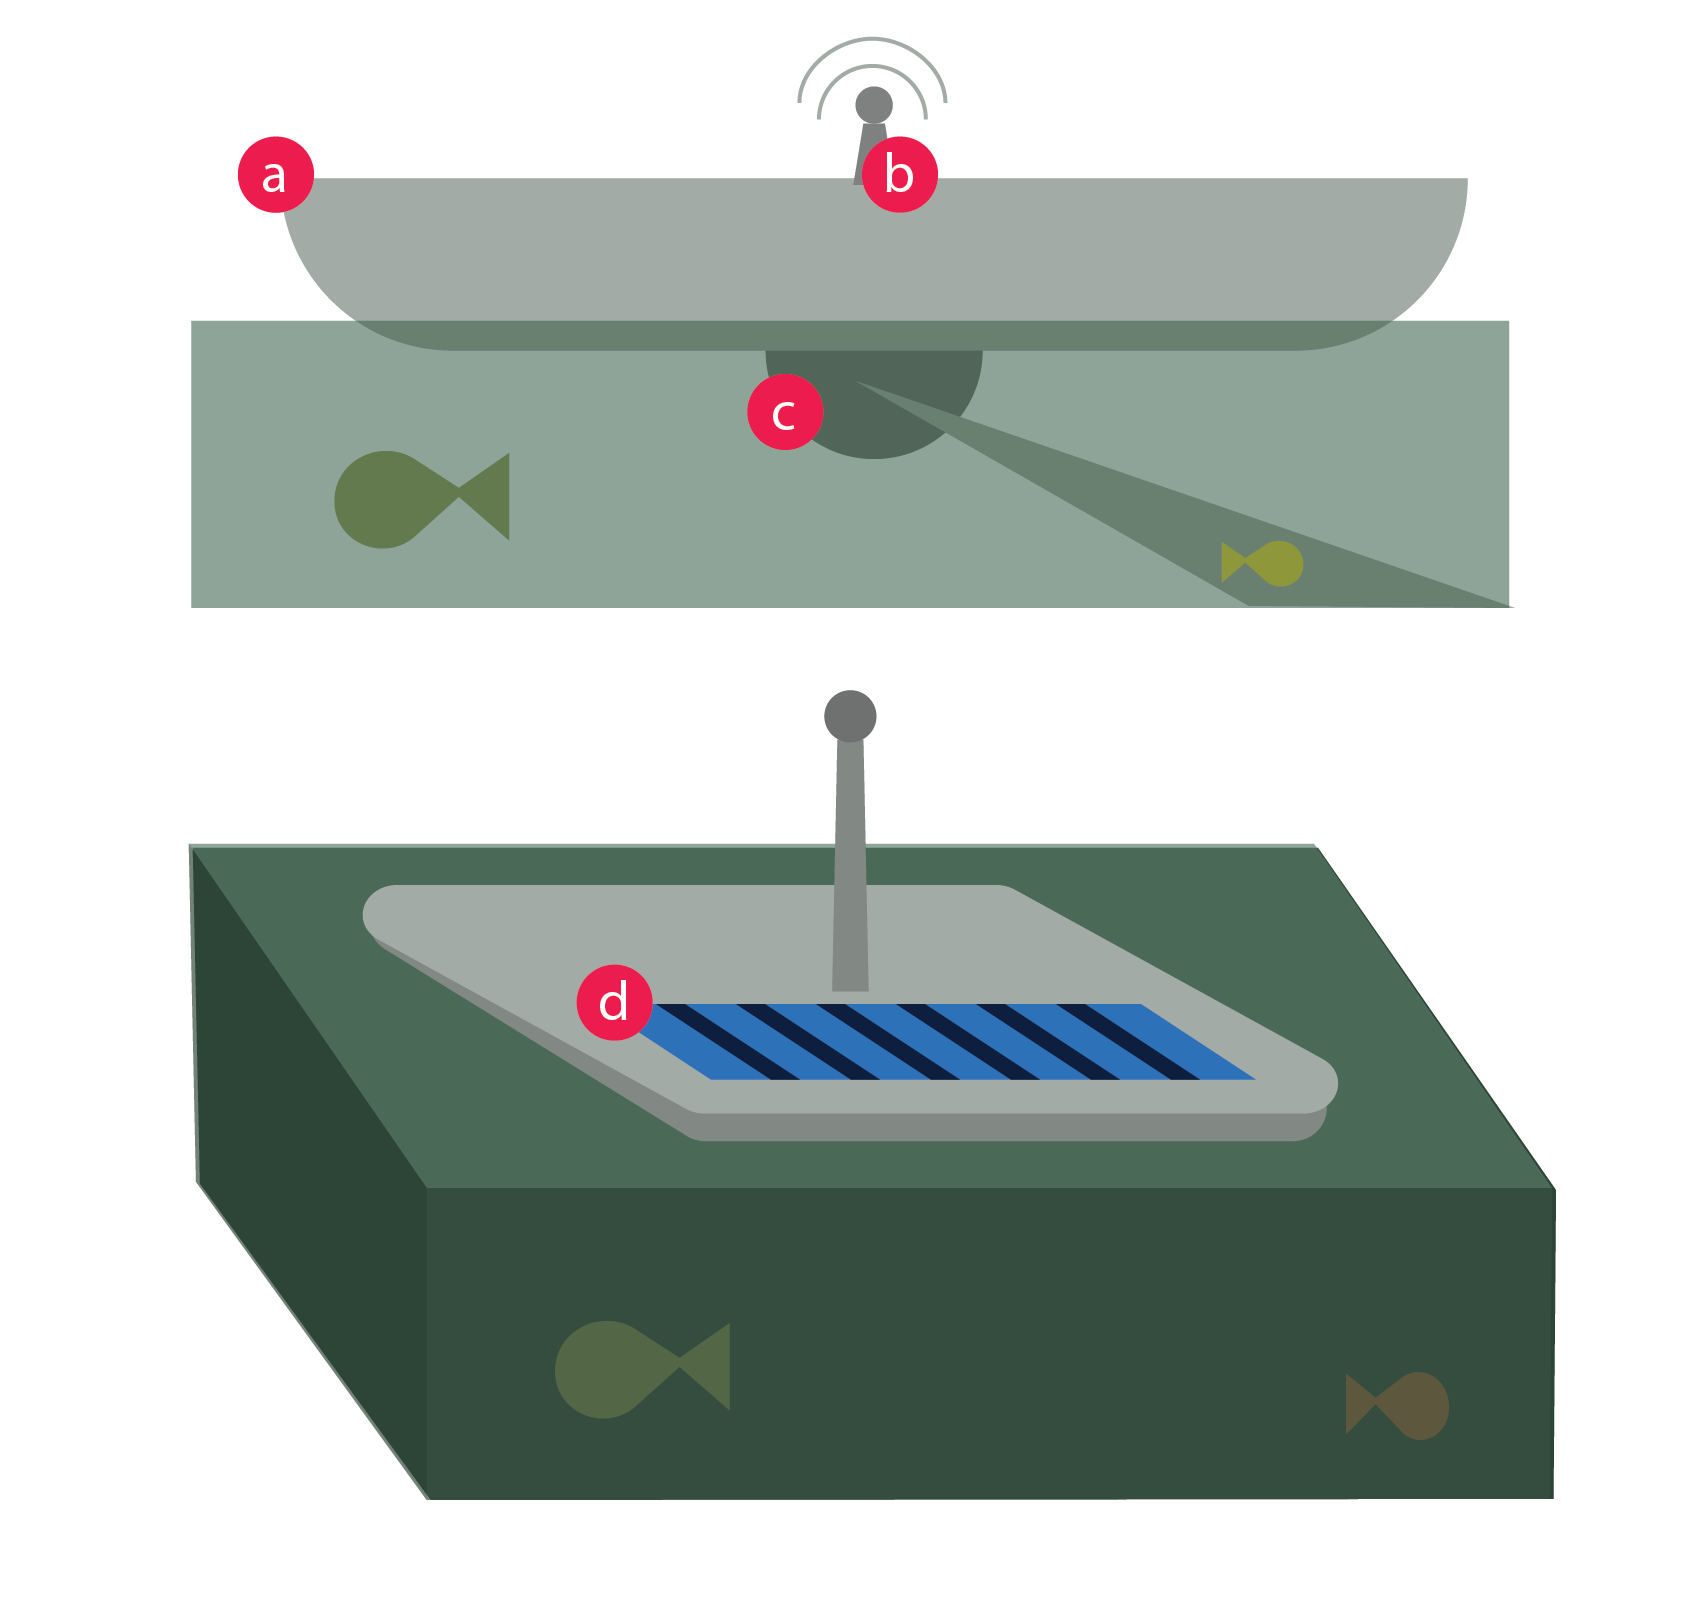
\includegraphics[width = 0.5\textwidth]{resources/blueprint.png}
    \legend{Fonte Própria}
\end{figure}

Como ilustra a \autoref{fig:blueprint}, os principais pontos a serem observados na construção da Boia são os seguintes:
\begin{description}
    \item[a.] Corpo da boia: será feito com materiais de baixo custo e de fácil acesso. Está será uma parte importante, uma vez que todos os componentes elétricos da boia estarão armazenados nesse contêiner. Sensores como:
    \begin{itemize}
        \item Placa de circuito integrado (\textit{Single Board Computer}: a placa definida para o projeto será uma variação do \textit{Raspberry Pi zero}\footnote{<https://www.raspberrypi.org/products/raspberry-pi-zero/>}, a \textit{Raspberry Pi zero W} \footnote{<https://www.raspberrypi.org/products/raspberry-pi-zero-w/>}, que por ter conexão \textit{wireless} embutida por padrão, diminuindo os custos com extensão para tal finalidade. 
        \item Sensor de captura óptica (câmera).
    \end{itemize}
    
    \item[b.] Sensor de captura óptica (câmera):  será utilizada a câmera \textit{Raspberry Pi Camera Module v2} \footnote{<https://www.raspberrypi.org/products/camera-module-v2/>}
    \item[c.] Antena: a antena que será utilizada no projeto está embutida no computador de placa única \textit{Raspberry Pi zero W}. 
    \item[d.] Placa Solar: será um painel solar (genérico) que irá alimentar parte do sistema.
\end{description}


%\section{A Boia no futuro}
%Com a possibilidade da adição de extensões à Boia, como sensores de medição de oxigenação da água, a necessidade de analise desses é algo pertinente para o desempenho da boia.

%\section{Identificação de Objetos utilizando openCV}
%O método utilizado para nessa primeira fase de identificações consiste nas seguintes etapas. Como mostra a Figura~\ref{fig:fluxfish} 



%\subsection{Pré-processamento}
%O pré-processamento da imagem é feito com a correção de cores, alterando seu sistema de cores de RGB para BGR como pode ser visto na figura~\ref{fig:fishp1}. 
%\begin{figure}[H]
%	\caption{\label{fig:fishp1} Alteração do sistema de cores para RGB}
%	\centering
%		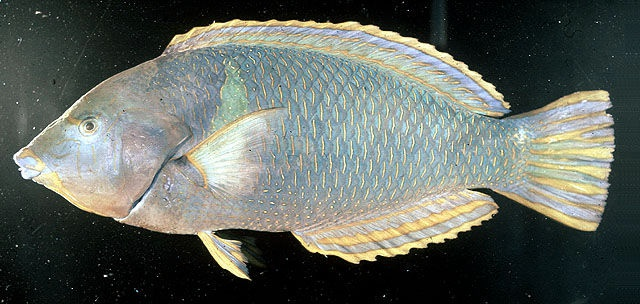
\includegraphics[width = 0.4\textwidth]			{fishes/fish_P1}
 %   \legend{Fonte Própria}
%\end{figure} 
%Para remoção de ruídos um filtro Gaussiano com outra modificação no sistema de cores é aplicado, facilitando a identificação de alguns pontos na imagem. o resultado pode ser visto na figura~\ref{fig:fishp2} 
%\begin{figure}[H]
%	\caption{\label{fig:fishp2} Aplicação de filtro Gaussiano e alteração do sistema de cores para HSV}
%	\centering
%		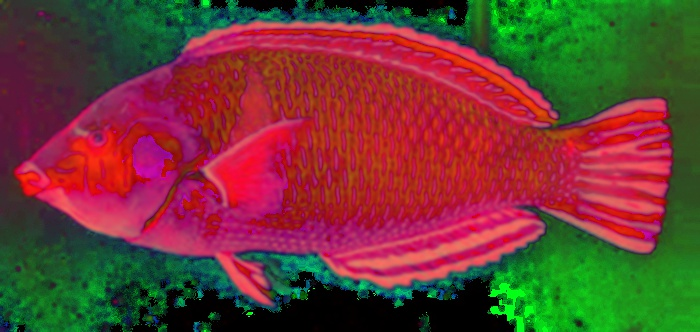
\includegraphics[width = 0.4\textwidth]			{fishes/fish_P2}
 %   \legend{Fonte Própria}
%\end{figure} 

%Em seguida a imagem deve ser livradas de alguns ruídos, assim um filtro gaussiano e conversão do sistema de cores serão aplicados. Resultado na Figura~\ref{fig:fishp2} 


%\subsection{Segmentação e identificação de objetos}
%A máscara de segmentação é baseada nos níveis de cores encontrados na imagem. Dois filtros são criados com espectros de cores diferentes e em seguida mesclados. . o resultado pode ser visto na figura~\ref{fig:fishp3_mask1}, a figura~\ref{fig:fishp5} mostra a exclusão de segmentos não necessários.
%\begin{figure}[H]
%	\caption{\label{fig:fishp3_mask1} Extração das máscaras}
%	\centering
%		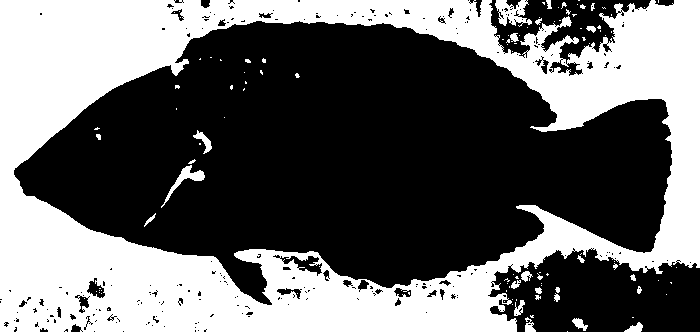
\includegraphics[width = 0.4\textwidth]			{fishes/fish_P3_mask1}
%    \legend{Fonte Própria}
%\end{figure}
%\begin{figure}[ht]
%	\caption{\label{fig:fishp5} Exclusão de segmentos}
%	\centering
%		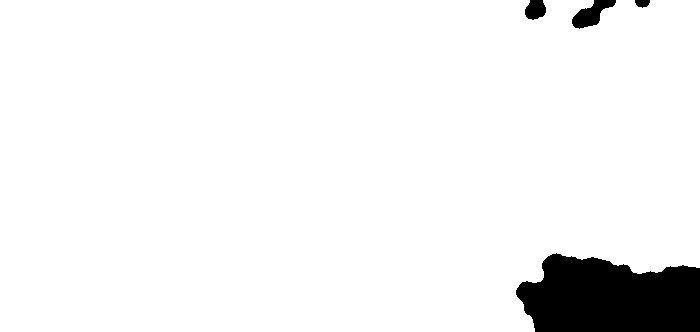
\includegraphics[width = 0.4\textwidth]			{fishes/fish_P5_mask_fishes}
 %   \legend{Fonte Própria}
%\end{figure} 

%A identificação de objetos na imagem é realizada através da identificação dos maiores pontos encontrados nas máscaras de segmentação, então esses são circulados, gerando a imagem de saída.
%\begin{figure}[H]
%	\caption{\label{fig:fishp5} Saída}
%	 \centering
%		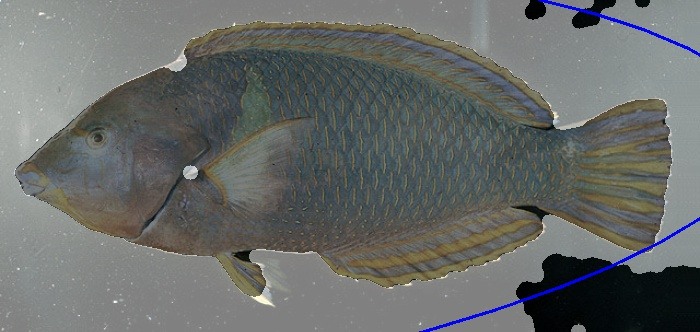
\includegraphics[width = 0.6\textwidth]			{fishes/fish_P7}
%    \legend{Fonte Própria}
%\end{figure}



